%iffalse           
\let\negmedspace\undefined
\let\negthickspace\undefined
\documentclass[journal,12pt,onecolumn]{IEEEtran}
\usepackage{cite}
\usepackage{amsmath,amssymb,amsfonts,amsthm}
\usepackage{algorithmic}
\usepackage{graphicx}
\usepackage{textcomp}
\usepackage{xcolor}
\usepackage{txfonts}
\usepackage{listings}
\usepackage{enumitem}
\usepackage{mathtools}
\usepackage{gensymb}
\usepackage{comment}
\usepackage[breaklinks=true]{hyperref}
\usepackage{tkz-euclide} 
\usepackage{listings}
\usepackage{gvv}                                        
\def\inputGnumericTable{}                                 
\usepackage[latin1]{inputenc}                                
\usepackage{color}                                            
\usepackage{array}                                            
\usepackage{longtable}                                       
\usepackage{calc}                                             
\usepackage{multirow}                                         
\usepackage{hhline}                                           
\usepackage{ifthen}                                           
\usepackage{lscape}

\newtheorem{theorem}{Theorem}[section]
\newtheorem{problem}{Problem}
\newtheorem{proposition}{Proposition}[section]
\newtheorem{lemma}{Lemma}[section]
\newtheorem{corollary}[theorem]{Corollary}
\newtheorem{example}{Example}[section]
\newtheorem{definition}[problem]{Definition}
\newcommand{\BEQA}{\begin{eqnarray}}
\newcommand{\EEQA}{\end{eqnarray}}
\newcommand{\define}{\stackrel{\triangle}{=}}
\theoremstyle{remark}
\newtheorem{rem}{Remark}
\usepackage{circuitikz}
\begin{document}

\bibliographystyle{IEEEtran}
\vspace{3cm}
\title{Assignment-4}
\author{EE224BTECH11044 - Muthyala Koushik% <-this % stops a space
}
\maketitle

\textbf{\section{Intersection of Conics}}

\textbf{Question:} Using integration, find the area of the region bounded by the line $y = 3x +2$, the $x-axis$ and the ordinates $x=-2$ and $x=1$ \\ 

\solution 

\begin{figure}[h!]
	\centering
	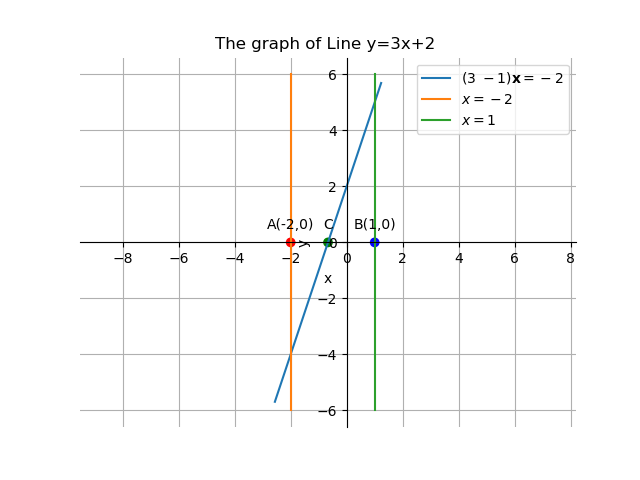
\includegraphics[width=0.6\linewidth]{figs/fig-1.png}
	\caption{The plot of the Line $y=3x+2$}
\end{figure}
  $y=3x+2 \iff \brak{3 -1}x=-2$ \\
  Let $\vec{C}\myvec{a\\0}$ be the point on $y=3x+2$ on $x$-axis:\\
   \begin{align}
       \brak{3 -1} \myvec{a \\ 0} = -2 \\
	   3a = -2 \iff a = -\frac{2}{3}
   \end{align}
 area of the $y=3x+2$ between lines x=-2 and x=1 is given by $A=A_1+A_2$ \\
$A_1$:Area from $x=-2$ to $x=-2/3$, $A_2$:Area from $x=-2/3$ to $x=1$
    \begin{align}
	    A &= \int_{-2}^{-\frac{2}{3}} \abs{3x + 2}  dx + \int_{-\frac{2}{3}}^{1} \abs{3x + 2}  dx \\
            A &= \int_{-2}^{-\frac{2}{3}} -\brak{3x + 2}  dx + \int_{-\frac{2}{3}}^{1} \brak{3x + 2}  dx \\
            A &= \sbrak{-\brak{\frac{3}{2}x^2 + 2x}}_{-2}^{-\frac{2}{3}} + \sbrak{\brak{\frac{3}{2}x^2 + 2x}}_{-\frac{2}{3}}^{1} \\
            A &= \brak{\frac{2}{3} - \brak{-2}} + \brak{\frac{7}{2} - \brak{-\frac{2}{3}}} \\
            A &= \brak{\frac{2}{3} + 2} + \brak{\frac{7}{2} + \frac{2}{3}} \\
            A &= \frac{8}{3} + \frac{25}{6} \\
            A &= \frac{41}{6}
    \end{align}
The area of the region bounded is $\frac{41}{6}$
\end{document}
